\chapter{Introduction to Spreadsheets}

For many real-world problems, spreadsheets are the perfect
tool. In this chapter, you will be introduced to how to use a
spreadsheet. There are numerous spreadsheet programs: Google Sheets,
Microsoft Excel, Apple Numbers, OpenOffice Calc, etc.  All of them are
very similar. I will be using Google Sheets, but if you are using one
of the others, you should be able to follow along.

The first spreadsheet program (VisiCalc) was introduced in 1979 as a
tool for finance people to play ``what if'' games.  For example, a
company might make a spreadsheet that told them how much more profit
they would make if they changed from using an expensive metal to using
a cheaper alloy.\index{Spreadsheet}

In honor of its history, let's start by studying a business question:
I have a friend who dreams of quitting her job to become a cooper. (A
cooper makes barrels that are used for aging wine and whiskey.)  She
says:
\begin{itemize}
\item It costs \$45 dollars in materials to build one barrel.
\item A barrel sells for \$100 dollars.
\item The workshop/warehouse she wants to rent costs \$2000 per month.
\item Taxes would take about 20\% of her profits
\item She needs to make \$4000 after taxes to live 
\end{itemize}

She has asked you, ``How many barrels do I need to make each month to survive?''

\section{Solving It Symbolically}

Many problems can be solved two ways: symbolically or
numerically.\index{symbolic vs. numeric solutions} To solve this
problem symbolically, you would write out the facts as equations or
inequalities and then do symbol manipulations until you ended up with
an answer. In this case, you would let $b$ be the number of barrells
and create the following inequality:

$$(1.0 - 0.2)\left(b(100 - 45) - 2000\right) \geq 4000$$

You would simplify it:

$$(0.8)\left(55 b - 2000\right) \geq 4000$$

And simplify it more:

$$44b - 1600 \geq 4000$$

If that is true, then:

$$44b \geq 5600$$

And if that is true, then:

$$b \geq \frac{1400}{11}$$

$1400/11$ is about 127.27, so she needs to make and sell 128 barrels
each month.

That is a perfect answer, and we didn't need a spreadsheet at all. Two things:
\begin{itemize}
\item As problems get larger and more realistic, it gets much more difficult to solve them symbolically.
\item As soon as you say ``Yes, you need to make and sell 128 barrels
  each month.'' Your friend will ask ``What if I make and sell 200
  barrels? How much money will I make then?''
\end{itemize}

So we will use a spreadsheet to solve the problem numerically.

\section{Solving It Numerically (with a spreadsheet)}


Let's get back to our example. Put labels in the A column:
\begin{itemize}
\item{Barrels produced (per month)}
\item{Materials cost (per barrel)}
\item{Sale price (per barrel)}
\item{Pre-tax earnings (per month)}
\item{Taxes (per month)}
\item{Take home pay (per month)}
\end{itemize}

Format them any way you like. It should look something like this:

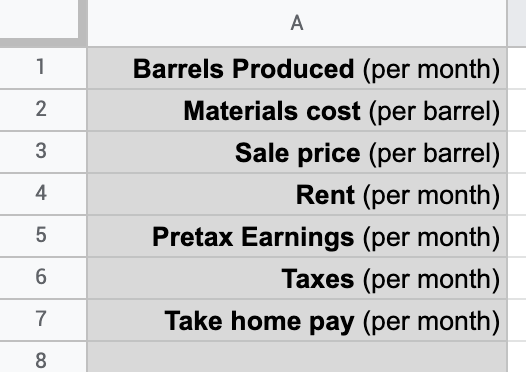
\includegraphics[width=0.4\textwidth]{BarrelLabels.png}

In the B column, the first four cells are values (not formulas):
\begin{itemize}
\item{115 formatted as a number with no decimal point}
\item{45 formatted as currency}
\item{100 formatted as currency}
\item{2000 formatted as currency}
\end{itemize}

It should look something like this:

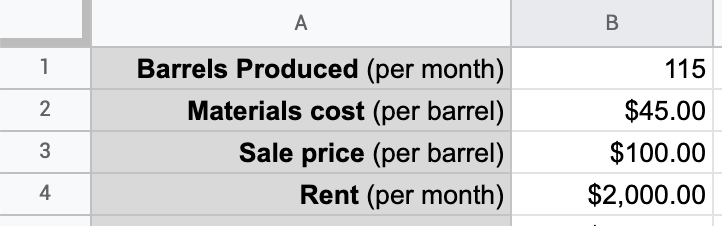
\includegraphics[width=0.5\textwidth]{BarrelValues.png}

The next three cells in the B column will have formulas:
\begin{itemize}
\item{B1 * (B3 - B2) - B4}
\item{0.2 * B5}
\item{B5 - B6}
\end{itemize}

It should look something like this:

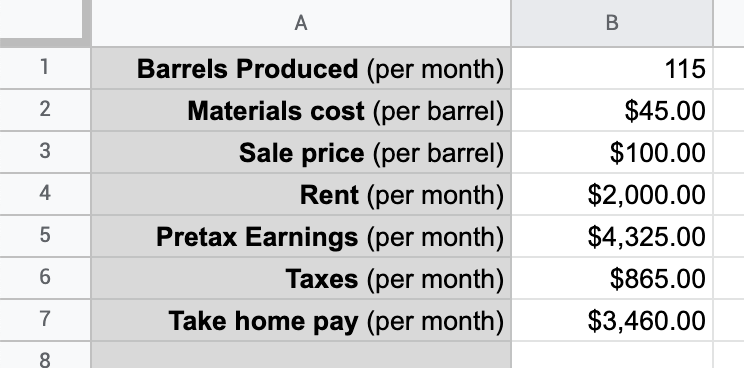
\includegraphics[width=0.5\textwidth]{BarrelFormulas.png}

Now you can share this spreadsheet with your friend and she can put
different values into the cells for what-if games.  Like ``If I can
get my materials cost down to \$42 per barrel, what happens to my take
home pay?''

Sometimes it is nice to show a range of values for a variable or two.
In this case, it might be nice to show your friend what the numbers
look like if she produces 115, 120, 125, 130, 135, or 140 barrels per
month.

We have one column, and now we need six. How do we duplicate cells?
\begin{enumerate}
\item Click B1 to select it and then shift click on B7 to select all seven cells.
\item Copy them. (There is probably a menu item for this.)
\item Click C1 to select it
\item Paste them.
\end{enumerate}

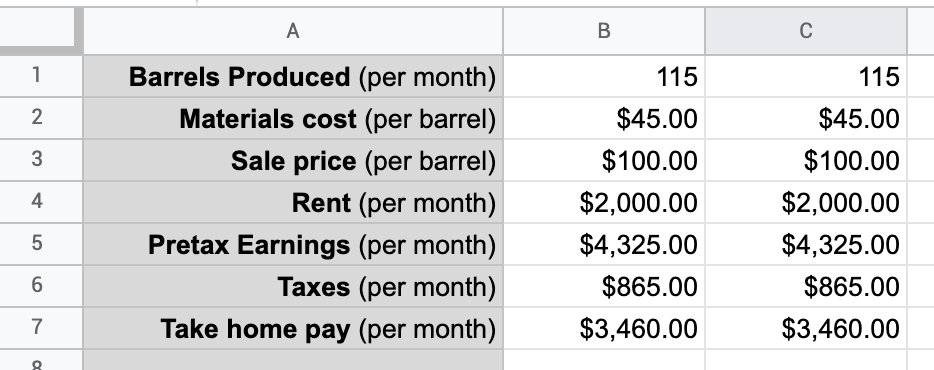
\includegraphics[width=0.5\textwidth]{BarrelCopyPaste.png}

We want the first cell in the new column to be 120. You could just
type in 120, but lets do something more clever.  Put a formula into that
cell: = B1 + 5.  Now the cell should show 120.

Why did we put in a formula? When we duplicate this column, this cell
will always have 5 more barrels than the cell to its left.

Now lets duplicate the second column a few times. The easy way to do
this is to select the cells as you did before and drag the lower-right
corner to the right until column G is in the selection. When you end
the drag, the copies will appear:

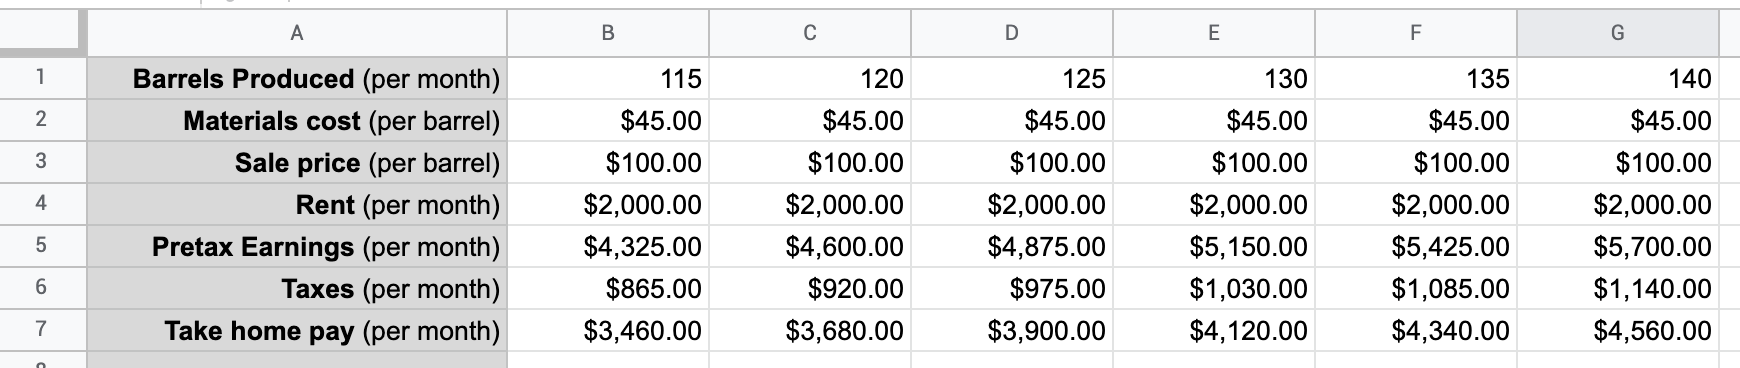
\includegraphics[width=0.8\textwidth]{BarrelDragPaste.png}

Nice, right? Now your friend can easily see how many barrels
corresponds to how much take-home pay. You know what she really wants? A graph.

\section{Graphing}

Graphing is a little different on every different platform.  Here is what you want the graph to look like.

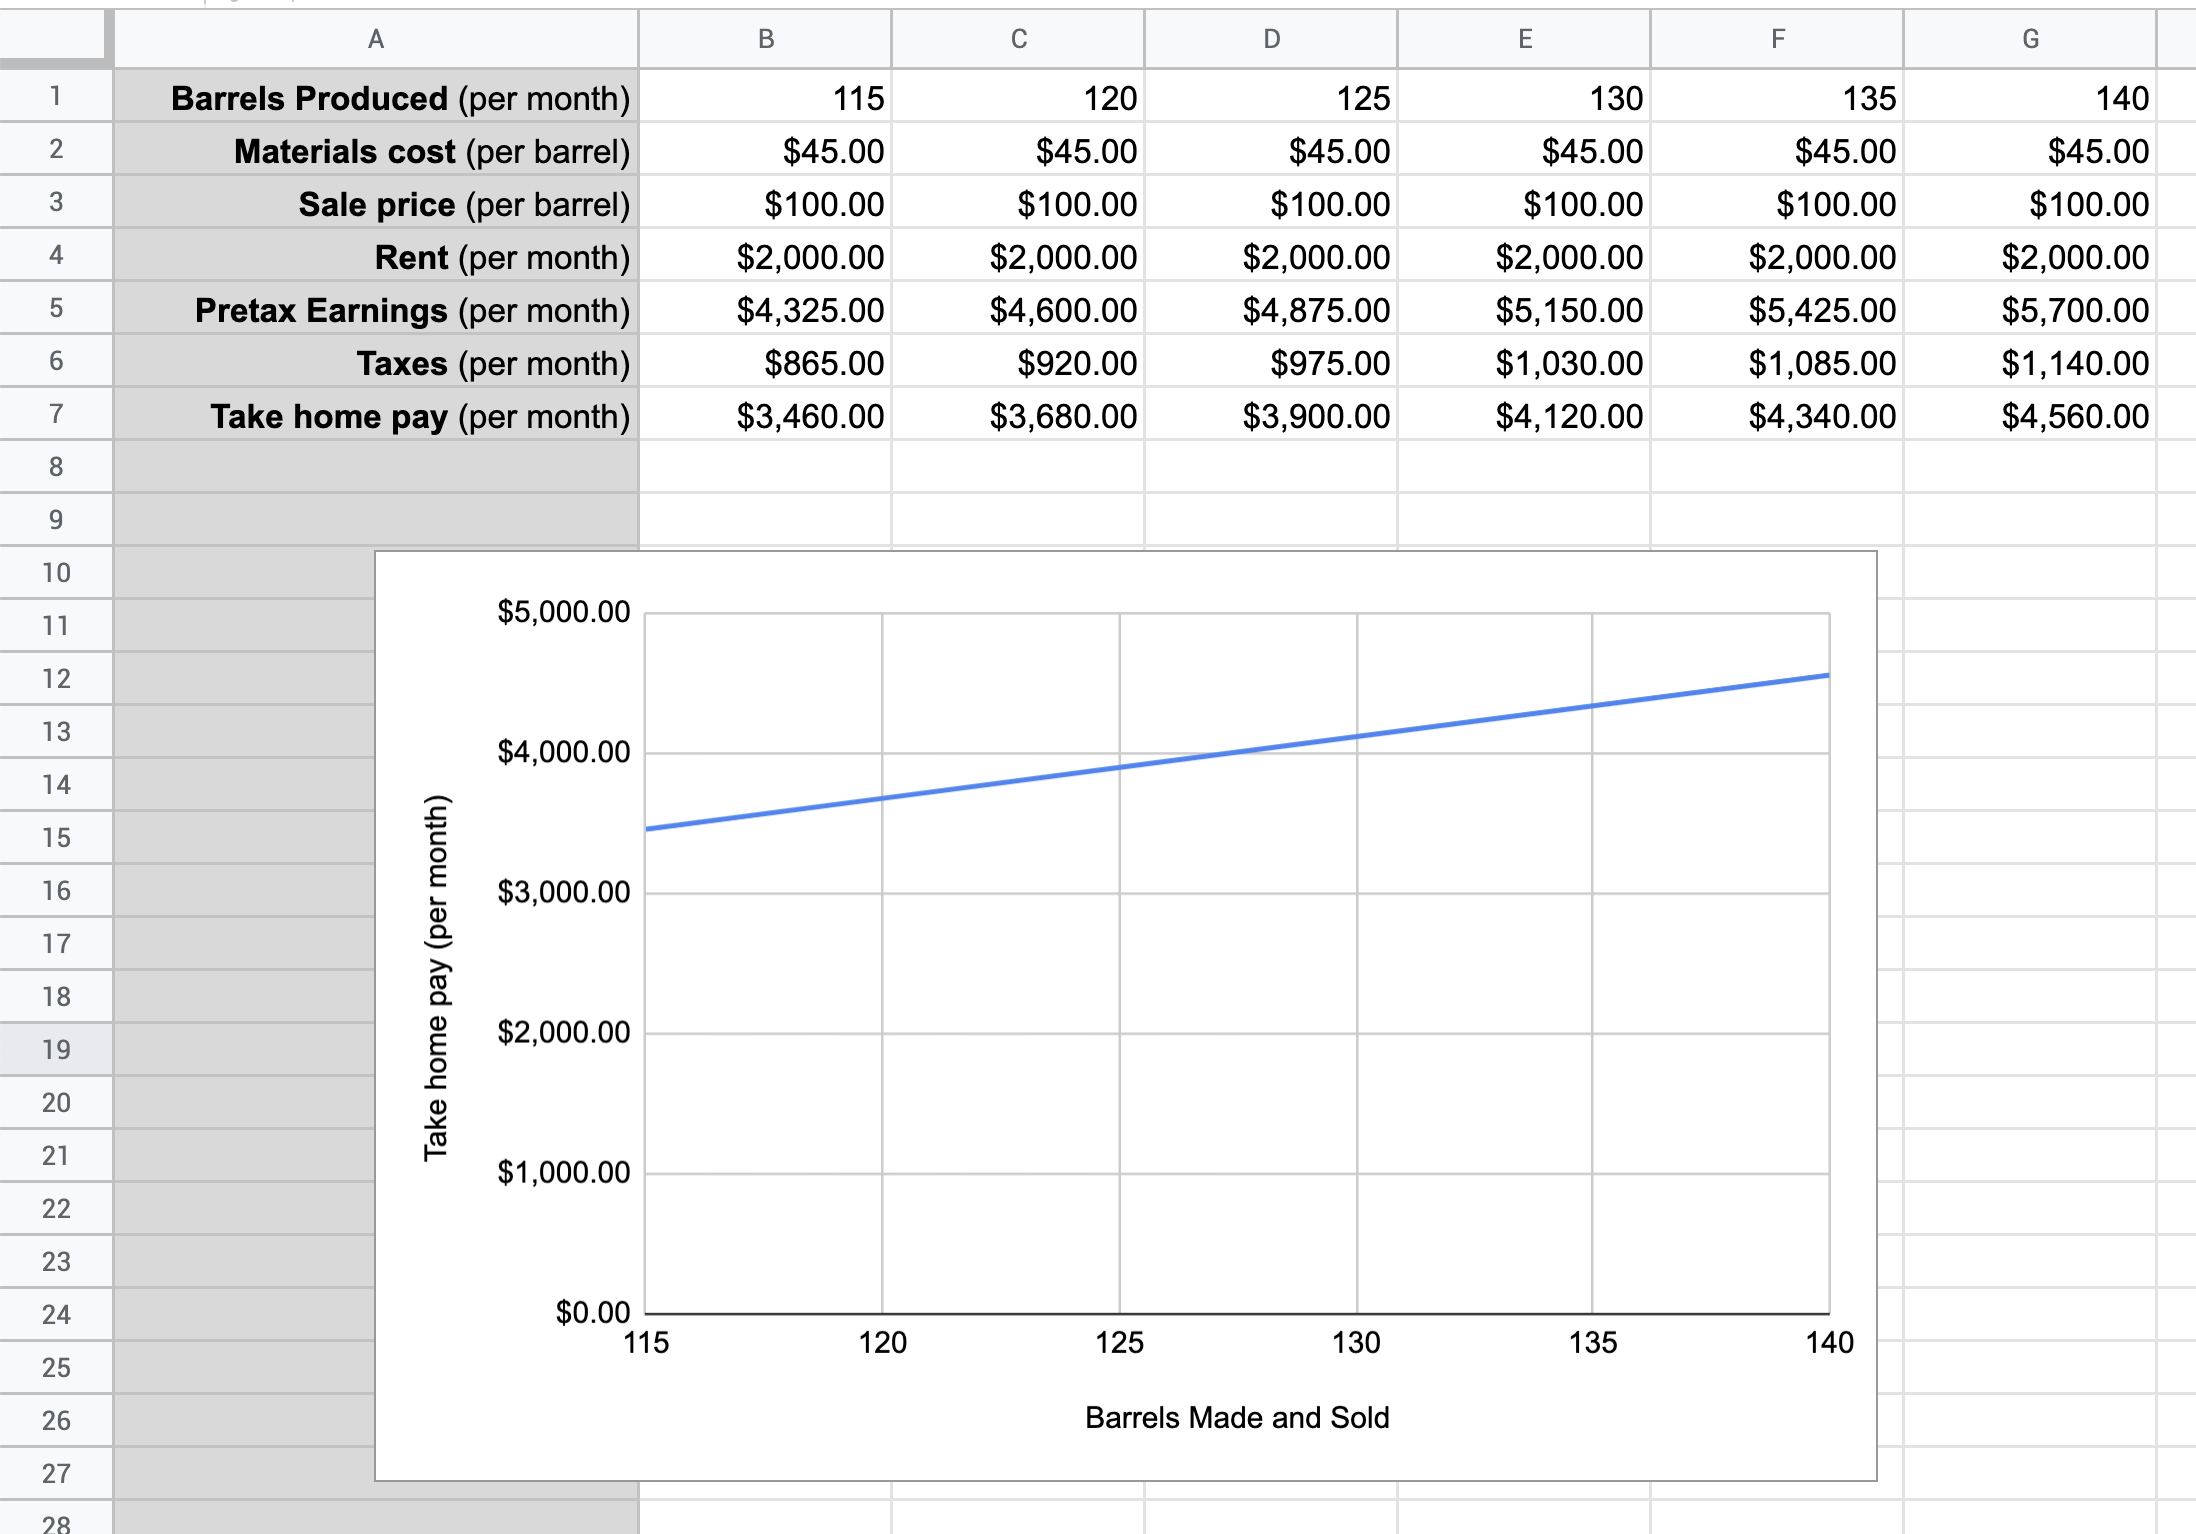
\includegraphics[width=0.8\textwidth]{BarrelGraph.png}

On Google Sheets:\index{spreadsheet!graphs}

\begin{enumerate}
\item Select cells B7 through G7. 
\item Choose the menu item Insert -> Chart.
\item Choose the chart type (Line)
\item Add the X-axis to be B1 through G1.
\item Under the Customize tab, Set the label for the X-axis to be ``Barrels Made and Sold''.
\item Delete the chart title (which is the same as the Y-axis label).
\end{enumerate}

\section{Other Things You Should Know About Spreadsheets}

Your spreadsheet document can have several ``Sheets''.  Each has its
own grid of cells.  The sheet has a name; usually you call it
something like ``Salaries''.  When you need to use a value from the
``Salaries'' sheet in another sheet, you can specify ``Salaries!A2''
-- that is, cell A2 on sheet ``Salaries''.  To flip between the sheets
there is usually a tab for each at the bottom of the document.

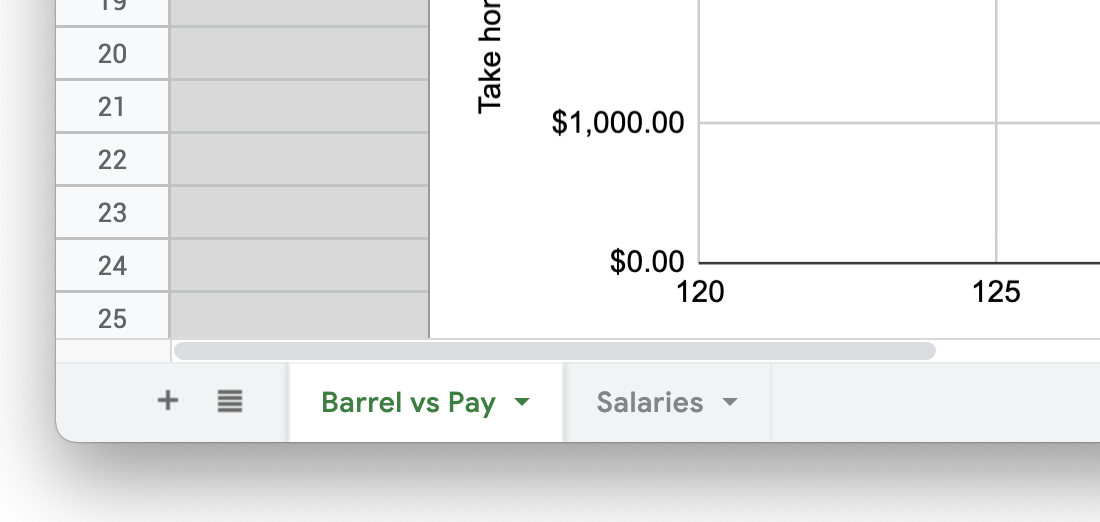
\includegraphics[width=0.5\textwidth]{Sheets.png}

By default, the cell references are relative.  That is, when you write
a formula in cell H5 that references the value in cell G4, the cell
remembers ``The cell that is one up and one to the left of me.''
Thus, if you copy that formula into B9, now that formula reads the
value from A8.

If you want an absolute reference, you use \$.  If H5 references
\$G\$4, G4 will be used no matter where on the sheet the formula is
copied to.

You can use the \$ on the row or colum.  In \$A4, the column is
absolute and the row is relative.  In A\$4, the row is absolute and
the column is relative.

\section{Challenge: Make a spreadsheet}

You have a company that bids on painting jobs. Make a
spreadsheet to help you do bids. Here are the parameters:
\begin{itemize}
\item The client will tell you how many square meters of wall need to be painted.
\item Paint costs \$0.02 per square meter of wall to cover
\item On average, a square meter of wall takes 0.02 hours to paint.
\item You can hire painters at \$15 per hour.
\item You add 20\% to your estimated costs for a margin of error and profit.
\end{itemize}

Make a spreadsheet such that when you type in the square meters to be
painted, the spreadsheet tells you how much you will spend on paint
and labor.  It also tells you what your bid should be.
